\documentclass[utf8]{ctexart}
\usepackage{xcolor} % 提供颜色支持
\usepackage{tikz}   % 用于绘图
\usepackage{pgfplots}%PGFPLOTS 是基于 TikZ 的专业绘图宏包
\begin{document}

% 示例1:将“家”字改为绿色
这是一个\textcolor{green}{家}的例子。
\pagestyle{plain}%为了使章节的页脚明确正确
% 示例2:绘制一个红色线段

\begin{tikzpicture}%tikzpicture 环境是 TikZ 宏包提供的核心绘图环境
    \draw[red, ultra thick] (0,0) -- (5,0); % 绘制从(0,0)到(5,0)的红色粗线
\end{tikzpicture}
%绘制一个三角形和矩形
\\
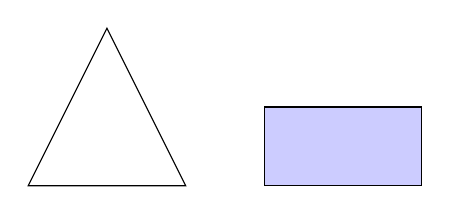
\begin{tikzpicture}
    \\
    \draw (0,0) -- (2,0) -- (1,2) -- cycle; % 三角形
    \\
    \draw[fill=blue!20] (3,0) rectangle (5,1); % 20:80的浅蓝色填充矩形
\end{tikzpicture}

\begin{tikzpicture}[domain=0:2*pi, samples=100]
    \draw[->] (-3.5,0) -- (7,0) node[right] {$x$};%x轴的绘制,符号标注x
    \draw[->] (0,-1.5) -- (0,1.5) node[above] {$y$};%y轴的绘制,符号标注y
    \draw[blue, thick] plot (\x, {sin(\x r)}); % 正弦函数%plot 是TikZ 的绘图命令,用于绘制函数曲线或离散数据点。
\end{tikzpicture}

\begin{tikzpicture}
    \draw (0,0) node[below left] {$A$} -- %在下方左侧添加数学标注 $A$
          (2,0) node[below right] {$B$} -- 
          (1,2) node[above] {$C$} -- cycle;
\end{tikzpicture}


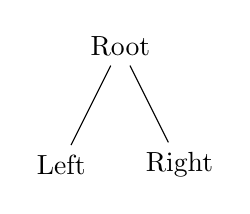
\begin{tikzpicture}[level distance=1.5cm]
    \node {Root}%二叉树
        child {node {Left}}
        child {node {Right}};
\end{tikzpicture}
\\
\\
\\
\begin{tikzpicture}
\begin{axis}[
    axis lines=middle,
    xlabel=$x$, ylabel=$y$,
    xmin=0, xmax=10, ymin=-1.5, ymax=1.5,
    xtick={0,1.57,3.14,4.71,6.28,7.85,9.42},
    xticklabels={$0$,$\frac{\pi}{2}$,$\pi$,$\frac{3\pi}{2}$,$2\pi$,$\frac{5\pi}{2}$},
    samples=100
]
    \addplot[blue, thick] {sin(deg(x))}; % PGFPLOTS 默认用度数,需用 deg() 转换
\end{axis}
%PGFPLOTS 默认使用度数作为角度单位,而 TikZ 默认使用弧度,使用deg(x)用于计算角度 x(以度数为单位)的正弦值
\end{tikzpicture}
\end{document}